%Para este capítulo se usará la abreviatura "conex".
\chapter{Conexión}
\label{conex}
La noción de conexión es otra más de las nociones que ya conocíamos en $\R^n$ y espacios métricos en general y que pueden generalizarse a un espacio topológico arbitrario. En este capítulo formalizaremos la noción intuitiva de estar hecho ``de una sola pieza''. Asimismo también trabajaremos sobre el concepto de ``pieza indivisible'' de algo, o, dicho más finamente, ``componente conexa''. 
\section{Definición y propiedades}
Comencemos nuestra nueva andadura definiendo formalmente la idea de conexión y presentando algunos resultados bastante potentes.

\begin{defi}[Conexión]
	Un espacio topológico $(\X,\T)$ es \tbi[espacio!conexo|see{conexo}]{conexo} \indexg{conexo} si no lo podemos particionar con dos abiertos. Dicho de otra manera, un espacio es conexo si no unión de dos abiertos disjuntos no vacíos.
	
	Escrito de forma conjuntista, no existen $\U$ y $\V$ abiertos tales que $U\cap V=\emptyset$ y $\X=U\cup V$.
\end{defi}

\begin{obs}[Conexión en subespacios]
	De nuevo, como ocurría con la compacidad, la conexión en un subconjunto no necesita una definición alternativa. En efecto, dado un subespacio $\Y\subset\X$, diremos que $\Y$ es conexo si lo es entendido como un espacio topológico equipado con la topología relativa.
\end{obs}
La siguiente proposición bien podría ser una observación inmediata, no obstante es extremadamente útil y nos acerca a la idea que de vez en cuando hemos dejado caer acerca a la relación de los clopens con la conexión.
\begin{prop}[Definiciones equivalentes]
	Sea un espacio topológico $\X$. Las siguientes afirmaciones son equivalentes:
	\begin{enumerate}
		\item $\X$ no es conexo.
		\item $\X$ es unión de dos cerrados disjuntos no vacíos.
		\item $\X$ posee dos clopens no triviales.
	\end{enumerate}
\end{prop}
\begin{proof}
	Si $\X$ es disconexo es claro que podemos escribir $\X$ como unión disjunta de dos abiertos no triviales $\X=U\cup V$. Como $U$ es abierto, su complementario, $V$, será cerrado, luego $V$ será un clopen. Análogamente, como $V$ es abierto, su complementario, $U$, será cerrado, luego $U$ es también un clopen.
\end{proof}
Para ir calentando daremos una caracterización de los conexos de la recta real $\R$. La demostración de la siguiente proposición simplifica brutalmente a la que habitualmente se ve en la literatura y es debida a Diego Chicharro.
\begin{defi}[Intervalo]
	Un subconjunto no vacío $A\subset\R$ se dice \tbi{intervalo} si dados dos puntos $a,b\in A$ y un tercero $c\in\R$ que cumple que $a\leq c\leq b$, entonces $c\in A$. 
\end{defi}
\begin{prop}[Conexos de la recta]
	Un conjunto $A\subset \R$ es conexo si y solo si es un intervalo. 
\end{prop}
\begin{proof}
	Demostremos ambas implicaciones.
	\begin{enumerate}
		\item[\bra] Sea $A$ conexo de $\R$ que no sea un intervalo, entonces habrá dos puntos $a,b\in A$ para cuales podemos elegir un $c$ entre $a$ y $b$ tal que $c\not\in A$. Dicho esto, considerando los conjuntos $U:=(-\infty,c)\cap A$ y $V:=(c,\infty)\cap A$ es claro que son abiertos disjuntos de $A$ que cubren a $A$, luego $A$ no es conexo. 
		\item[\bla] Sea $A$ un intervalo. Si no fuera conexo, podría particionarlo en dos cerrados $F$ y $H$. Tomemos pues dos puntos, uno en cada abierto de la partición $a\in F$ y $b\in H$, supongamos sin pérdida de generalidad que $a<b$. Como $A$ es un intervalo, dados dos puntos de $A$, contiene a todos los que haya en medio, en particular $[a,b]\subset A$.
		
		Consideremos pues $H\cap[a,b]\not=\emptyset$, que, al ser intersección de cerrados es cerrado, y, por tanto, contiene a todos sus puntos de acumulación, en particular, al ser acotado contiene a su ínfimo, al que llamaremos $\eta$.
		
		Llegados a este punto, si $\eta=a$ entonces $a$ estará en los dos cerrados de la partición a la vez, lo cual es absurdo, precisamente por ser una partición. Esto obliga a que $\eta > a$, luego $[a,\eta)\cap H=\emptyset$ así que $[a,\eta)\subset F$. Al ser $F$ cerrado es claro que $[a,\eta]\subset F$. Pero esto es absurdo porque entonces $\eta$ estaría tanto en $F$ como $H$, que son conjuntos disjuntos.\qedhere
	\end{enumerate}
\end{proof}
Un corolario inmediato a esta proposición es que $\R$ es conexo, ya que $\R=(-\infty,\infty)$.

Ahora, vamos a repasar brevemente las propiedades que ya conocíamos de conjuntos conexos en espacios métricos que siguen siendo válidas en estos mundos abstrusos.

\begin{prop}[Imagen continua]
	\label{conex_prop_im_continua}
	La imagen continua de un conexo es un conexo.
\end{prop}
\begin{proof}
	Sea $\X$ conexo y $f:\X\to f(\X)=:\Y$ continua. Veamos que $\Y$ es conexo. Razonemos pues por contradicción.
	
	Si $\Y$ no fuera conexo, tendría un clopen no trivial (ni el vacío ni el total), llamémoslo $A$. Entonces por ser $f$ continua, $f^{-1}(A)$ también es un clopen.
	
	Al ser $f$ sobreyectiva, $f(f^{-1}(A))=A\subsetneq f(\X)$, luego $f^{-1}(A)$ no puede ser ni el vacío ni el total, siendo así un clopen no trivial, entrando en contradicción con la conexión de $\X$.
\end{proof}

A continuación presentamos un teorema conocido en algunos lugares remotos como el teorema del pivote, aunque bien podría llamarse el teorema MacGyver.
\begin{theo}[Teorema de pivote]
	\label{conex_theo_pivote}
	Sea $\{A_i\}_{i\in I}$ una familia de conexos de $\X$ con intersección no vacía, es decir, hay un punto $a$ contenido en $\bigcap_{i\in I} A_i$.
	
	Entonces, la unión de la familia, $C:=\bigcup_{i\in I} A_i$ es conexo.
\end{theo}
\begin{proof}
	Veamos que $C$ no tiene clopens no triviales, para ello, supongamos que $S$ es un clopen de $C$. Al ser $S$ un clopen de $C$, por topología relativa, $S\cap A_i$ es un clopen de $A_i$. Ahora, como $A_i$ es conexo, $S\cap A_i$ tiene que ser necesariamente el vacío o el total, para cada $i\in I$.
	
	Si hubiera un $i_0\in I$ tal que $S\cap A_{i_0}=A_{i_0}$, como hay un $a$ en la intersección de la familia, $a\in A_{i_0}$, luego $a\in S$. Por tanto $S$ corta a todos los conjuntos de la familia, y, como dijimos antes, es un clopen en todos ellos, luego no queda más remedio que $S\cap A_i=A_i$ para todo $i\in I$. Siendo pues $S=C$.
	
	Por otra parte, si $S$ no corta a ninguno de los conjuntos de la familia es claro que es el vacío. 
\end{proof}

Este teorema es extremadamente útil para garantizar la conexión de un sinnúmero de conjuntos, y genera un gran abanico de corolarios y consecuencias (de ahí que le hayamos bautizado como el teorema MacGyver). Detallemos algunas variantes y consecuencias de este fantástico teorema.

\begin{cor}[Intersecciones dos a dos]
	\label{conex_cor_pivote_corte_comun}
	Sea $\{A_i\}_{i\in I}$ una familia de conexos que cumple que uno de ellos, digamos $A_{i_0}$, corta a todos los demás. Es decir, $A_{i_0}\cap A_i\not=\emptyset$ para todo $i\in I$.
	
	Entonces, la unión de la familia, $\bigcup_{i\in I} A_i$ es conexo.
\end{cor}
\begin{proof}
	Como $A_i\cap A_{i_0}\neq\emptyset$ por hipótesis, podemos aplicar el teorema del pivote a la familia $\{A_i,A_{i_0}\}$ para cada $i\in I$, y por tanto cada $A_{i_0}\cup A_i$ es conexo. Ahora, escribiendo
	\[\bigcup_{i\in I} A_i = \bigcup_{i\in I} (A_i\cup A_{i_0})\]
	tenemos que como la familia $\{A_i\cup A_{i_0}\midc i\in I\}$ tiene a $A_{i_0}$ por intersección, su unión (que coincide con la que queremos), por el teorema del pivote es conexa.
\end{proof}
\begin{obs}[Intersecciones dos a dos]
	En particular, la misma prueba del corolario \ref{conex_cor_pivote_corte_comun} tomando un $i_0\in I$ arbitrario sirve para una familia de conexos tal que su intersección dos a dos sea no vacía, es decir, $A_i\cap A_j\not=\emptyset$ para cualquier par de conjuntos de la familia.
\end{obs}
Como a veces la visión espacial brilla por su ausencia brindamos dos dibujos con ejemplos de familias de conexos que verifican las condiciones del corolario \ref{conex_cor_pivote_corte_comun}.
\begin{figure}[h!]
	\centering
	\subfigure[El corro de la patata]{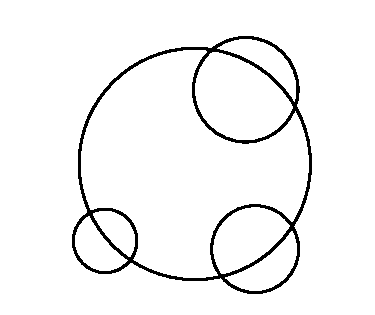
\includegraphics[scale = 0.4]{img/pivote_variante1}}\qquad\qquad
	\subfigure[El símbolo anarquista]{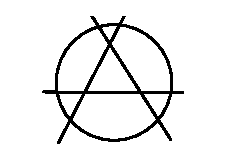
\includegraphics[scale = 0.8]{img/pivote_variante2}}
	\caption{Ilustración de conjuntos en las hipótesis de \ref{conex_cor_pivote_corte_comun}.}
\end{figure}

\begin{cor}[Cadenas]
	Sea una cadena finita $\{A_i\}_{i=1}^n$ de conexos, es decir, que verifica que $A_i\cap A_{i+1}\not=\emptyset$. Entonces $\bigcup_{i=1}^n A_i$ es conexo.
\end{cor}
\begin{proof}
	Por inducción, es claro que aplicando el teorema del pivote la cadena de dos eslabones $A_1\cup A_2$ es conexa, si suponemos que la cadena de $n$ eslabones es conexa, por el teorema del pivote, la de $n+1$ eslabones $A_{k+1}\cup\bigcup_{i=1}^k A_i$ lo será también.
\end{proof}
\begin{figure}[H]
	\centering
	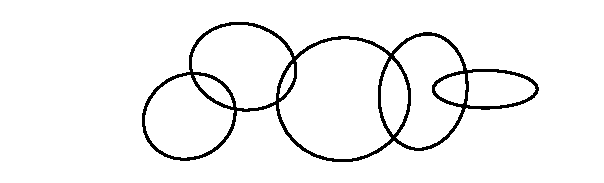
\includegraphics[scale = 0.5]{img/pivote_variante3}
	\caption{Ilustración de una cadena de conexos}
\end{figure}
\begin{obs}
	El corolario anterior también se verifica si la sucesión de conjuntos es numerable, pero no lo vamos a probar aquí.
	% AQUÍ VIENE PROBADO http://dbfin.com/topology/munkres/chapter-3/section-23-connected-spaces/problem-2-solution/
\end{obs}

El siguiente resultado, aunque también es consecuencia del teorema del pivote \ref{conex_theo_pivote}, es más que un mero corolario y merece la categoría de teorema por sí mismo.

\begin{theo}[Sandwich]\label{conex_teo_adherencia_conexa}
	Sea $A$ conexo y $B$ un conjunto emparedado entre $A$ y su adherencia, es decir, $A\subset B\subset\adher{A}$. Entonces $B$ es conexo. En particular, $\adher{A}$ es conexo.
\end{theo}
\begin{proof}
	Podemos poner nuestro conjunto $B$ de forma amigable para usar el teorema del pivote.
	\[B=\bigcup_{b\in B\setminus A} (A\cup\{b\}) \]
	como la intersección de la familia es no vacía, entonces basta probar que cada $A\cup\{b\}\subset\adher{A}$ es conexo, pues en ese caso el teorema del pivote \ref{conex_theo_pivote} nos garantiza la conexión de $B$.
	
	Si hubiera un clopen no trivial $C\subset A\cup\{b\}$, entonces, $C\cap A$ sería un clopen en $A$. Como $A$ es conexo, $C\cap A$ debe ser el vacío o el total.
	\begin{itemize}
		\item Si es el vacío, entonces $C=\{b\}$ y por tanto $\{b\}$ es abierto, luego, como el entorno $\{b\}$ de sí mismo no corta con $A$, $b\not\in\adher{A}$, lo cual es una contradicción.
		\item Si es el total, $C=A$ y por tanto $A$ es cerrado, pero $b\not\in A=\adher{A}$, que de nuevo es una contradicción. \qedhere
	\end{itemize}
\end{proof}

Recojamos los frutos de nuestra cosecha con un ejemplo, pero antes presentemos unas definiciones que harán más ágil nuestro discurrir.
\begin{defi}[Segmento]
	En $\R^n$ un segmento que une dos puntos $a$ y $b$ es el conjunto $\{ta+(1-t)b\midc t\in[0,1]\}$, que puede interpretarse como la imagen de la interpolación lineal entre $a$ y $b$, que definimos en la ecuación \eqref{interpolacion}.
\end{defi}
\begin{defi}[Convexo]
	En $\R^n$, se dice que un conjunto es \tbi{convexo} si para cada par de puntos $a,b\in E$, el segmento que los une también está en el conjunto.
\end{defi}
\begin{defi}[Estrellado]
	En $\R^n$ definimos conjunto \tbi{estrellado} como un conjunto en el que existe un punto tal que el segmento de él a cualquier otro está en el conjunto.
\end{defi}

\begin{exa}[Miscelánea]
	\label{conex_exa_miscel}
	Veamos algunos ejemplos de conjuntos conexos:
	\begin{enumerate}
		\item Los segmentos son conexos por ser la imagén continua de $[0,1]$, que es conexo, por la interpolación lineal, que es continua.
		\item Si un conjunto es convexo entonces es estrellado, y si es estrellado entonces es conexo. Además, las implicaciones recíprocas no se verifican. En resumen
		\[\text{Convexo}\ra\text{Estrellado}\ra \text{Conexo}\]
		
		En efecto, si $A$ es convexo tomando cualquier punto como ``centro de la estrella'' se deduce que $A$ es estrellado.
		
		Asimismo, si $A$ es estrellado se puede escribir como
		\[A=\bigcup_{a\in A} [a_0, a]\]
		para cierto $a_0\in A$. Cada segmento $[a_0,a]$ es conexo, y, por tanto, por el teorema del pivote, como todos comparten el punto $a_0$, su unión es conexa.
		
		Nótese que ni la convexidad ni ser estrellado son propiedades topológicas; ambas son propiedades vectoriales: su definición solo tiene sentido en un espacio que, al menos, tenga estructura de espacio vectorial.
		
		\item Una circunferencia en $\R^2$ es conexa, pero no es estrellada. En efecto, es conexa por ser la imagen de $[0,2\pi]$ por la aplicación $t\mapsto (\cos t, \sen t)$.
		
		\item El grafo de la función $\sen\frac{1}{x}$ para $x>0$, que escribimos:
		\[C = \left\{\left(x,\sen\frac{1}{x}\right)\midc x>0\right\}\]
		es conexo por ser la imagen continua de $(0,\infty)$ por la aplicación:
		\[x\mapsto \left(x,\sen\frac{1}{x}\right)\]
		
		Lo que es más interesante, para cualquier $a\in [-1,1]$ se verifica que $\{(0,a)\}$ es adherente a $C$ (es relativamente fácil de comprobar) y por tanto que $C\cup\{(0,a)\}$ es conexo.
		\begin{figure}[H]
			\centering
			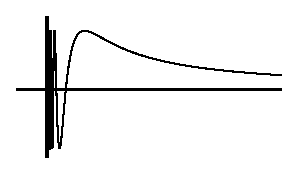
\includegraphics[scale = 0.8]{img/funcionsen1x}
			\caption{Ilustración de la gráfica de $\sen(1/x)$}
		\end{figure}
		
		\item Consideramos el conjunto:
		\begin{equation}\label{lineas}C = \big(\{0\}\times (0,1]\big) \cup \left(\bigcup_{n\in\N} [0,1]\times\left\{\frac{1}{n}\right\}\right) \end{equation}
		\begin{figure}[H]
			\centering
			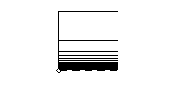
\includegraphics[scale = 0.2]{img/lineas}
			\caption{Ilustración del conjunto de la ecuación \eqref{lineas}}
		\end{figure}
		que es unión de segmentos horizontales cada vez más juntos y de un segmento vertical. Este es trivialmente conexo por el corolario \ref{conex_cor_pivote_corte_comun}. Lo particular es que si unimos a $C$ el segmento horizontal:
		\[(0,1)\times\{0\}\]
		sigue siendo conexo por ser adherencia de $C$ (¡compruébese!). 
\qedhere
	\end{enumerate}
\end{exa}

Completamos esta sección con una propiedad interesante garantizada por la conexión.

\begin{lem}[Cadena]
	Sea $\X$ conexo y $\{U_i\}_{i\in I}$ un recubrimiento por abiertos de $\X$. Dos puntos cualesquiera $x,y\in\X$ se pueden conectar mediante una cadena finita de abiertos del recubrimiento.
\end{lem}

\begin{proof}
	Sea $A=\{z\in\X \midc \text{existe una cadena de } x \text{ a } z \}$. $A$ es claramente no vacío, puesto que $x\in A$. Por ende, nuestro objetivo será ver que $\X=A$. Una forma de hacerlo será ver que $A$ es un clopen, ya que si lo fuera, por conexión de $\X$ y por ser $A$ no vacío $A$ tendría que ser el total.
	\begin{itemize}
		\item Veamos que $A$ es abierto. En efecto, dado $z\in A$, queremos ver que existe un abierto $U$ tal que $z\in U\subset A$. Si tomamos el último abierto $U$ de la cadena que une $x$ y $z$ hemos ganado, ya que $U\subset A$, ya que todo punto de $U$ queda unido con $x$ con la misma cadena que $z$.
		
		\item Ahora la clausura. En efecto, si $z\in\adher{A}$, entonces habrá un abierto $U_{i_0}$ tal que $U_{i_0}\cap A\not=\emptyset$. Considerando un punto $y$ de la intersección, como $y$ está en $A$, hay una cadena de $x$ a $y$. Uniendo $U_{i_0}$ a la cadena obtenemos una cadena de $x$ a $z$, y por tanto $z\in A$, luego $A=\adher{A}$. \qedhere
	\end{itemize}
\end{proof}
Este último resultado tiene una aplicación muy importante en los espacios euclídeos usuales.
\begin{defi}[Poligonal]
	Una \tbi{poligonal} en $\R^n$ es un conjunto $\Gamma$ de la forma\begin{equation*}
		\Gamma=[x_0,x_1]\cup[x_1,x_2]\cup\dots\cup[x_{n-2},x_{n-1}]\cup[x_{n-1},x_n]
	\end{equation*}
	Donde $[x_i,x_j]$ representa el segmento que une a los puntos $x_i$ y $x_j$. Nótese que por la variante de las cadenas del teorema del pivote una poligonal es conexa.
\end{defi}
\begin{defi}[Conexión por poligonales]
	Un conjunto $A\subset\R^n$ se dice \tbi[conexo!por poligonales]{conexo por poligonales} si dados dos puntos cualesquiera $x,y\in A$, hay una poligonal $\Gamma$ contenida en $A$ que une a $x$ y a $y$.
\end{defi}
\begin{obs}[Conexión y conexión por poligonales]
	Todo conjunto conexo por poligonales es conexo. En efecto, si tomamos un punto $a$ de $A$ y consideramos la familia de poligonales (conexos) que conectan a $a$ con el resto de puntos de $A$, tenemos que dicha familia tiene a $\{a\}$ por intersección, luego podemos aplicar el teorema del pivote, obteniendo que la unión de la familia, que es $A$, es conexa.
\end{obs}
\begin{obs}[Abiertos y conexión por poligonales]
	Podemos recubrir cualquier abierto conexo de $\R^n$ con bolas (véase el lema \ref{etop_lem_otrasProp}), y, por tanto existe una cadena de bolas que une cualquier par de puntos.
	
	Si tomamos un punto en cada intersección entre bolas consecutivas de la cadena y consideramos los segmentos que los unen, tengo una poligonal que conecta los dos puntos.
	
	De esta forma, para abiertos de $\R^n$ la conexión y la conexión por poligonales son nociones equivalentes.
\end{obs}

\section{Componentes conexas}

Al igual que ocurría con la compacidad, sería deseable que todos los espacios fuesen conexos. Dado que esto no se da, nos conformaremos con quedarnos con los subconjuntos conexos del espacio. Surge así la idea de componente conexa que definimos a continuación.

Aunque parezca que esto no es una ventaja, es tremendamente útil a la hora de estudiar, por ejemplo, si dos espacios son homeomorfos, ya que el número de componentes conexas se conserva por homeomorfismos (ver ejemplo \ref{etop_exa_homeomorfismos}).

\begin{defi}[Componente conexa de un punto]
	Se dice que un conjunto $\Co(x)\subset\X$ es una \tbi{componente conexa} de $x\in\Co(x)$ si es un conjunto conexo ``maximal''. Esto es que, dado un conjunto $D$ conexo que contiene a $x$ se verifica que $\Co(x)\not\subset D$.
	
	En general, diremos que un conjunto $\Co$ es una componente conexa si lo es de alguno de sus puntos (y por tanto de todos, véase la observación \ref{conex_obs_compartido}).
\end{defi}

Análogamente a lo que hicimos con el interior y la adherencia en el capítulo \ref{etop}, veamos que la componente conexa de un punto tiene una caracterización conjuntista muy sencilla.

\begin{lem}[Caracterización conjuntista]
	Dado $x\in\X$, el conjunto 
	$\Co(x)=\bigcup_{A\subset\X} A$ con $x\in A$ y $A$ conexo, es una componente conexa de $x$.
\end{lem}
\begin{proof}
	En efecto, $\Co(x)$ es no vacío, ya que $\{x\}$ es conexo. Además, la familia de conexos que conforma $\Co(x)$ tiene al menos a $\{x\}$ en la intersección, luego, por el teorema de pivote, $\Co(x)$ es conexo.
	
	Por construcción es, además, maximal, ya que, si hubiera un conexo que lo contuviera, este contendría a $x$, y, por tanto, estaría $\Co(x)$.
\end{proof}
\begin{obs}[Unicidad]
	\label{conex_obs_unicidad}
	Cabe destacar que $\Co(x)$ no es solo una componente conexa de $x$, sino \tb{la} componente conexa de $x$. 
	
	En efecto, si hubiera otra, digamos $E$, tanto $\Co(x)$ como $E$ deben contener a $x$, luego su intersección será no vacía $E\cap \Co(x)\not=\emptyset$. En tal caso, $A:=E\cup \Co(x)$ sería conexo por el teorema del pivote, y, como además $x\in A$, $A$ estará en la familia que conforma $\Co(x)$, luego $E\subset\Co(x)$. Como $E$ es una componente conexa se debe dar la igualdad.
\end{obs}
\begin{obs}[Intersección y contención]
	\label{conex_obs_inter}
	La observación \ref{conex_obs_unicidad}, a parte de darnos la unicidad de la componente conexa de un punto, nos viene a decir, que si un conexo corta a la componente conexa, este debe estar contenido en ella. Este hecho puede sacarnos de algún que otro apuro. 
\end{obs}
\begin{obs}[Componente conexa compartida]
	\label{conex_obs_compartido}
	Nótese que pudiera haber varios puntos con la misma componente conexa, de hecho, todos los puntos de $\Co(x)$ tienen a $\Co(x)$ por componente conexa. En efecto, sea $y\in\Co(x)$, llamemos $\Co(y)$ a su componente conexa. Es claro que, por la caracterización conjuntista $\Co(x)\subset\Co(y)$, luego, $x\in\Co(y)$, $\Co(y)$ es un conexo que contiene a $x$, por tanto, debe estar contenido en su componente conexa, es decir $\Co(y)\subset\Co(x)$.
	
	En definitiva podemos concluir que una componente conexa lo es de todos sus puntos y de ninguno más (obviamente). En particular, si un espacio es conexo, es la componente conexa de todos sus puntos.
\end{obs}

A continuación enunciamos y demostramos algunas propiedades de las componentes conexas.

\begin{lem}[Propiedades varias]
	Sea $\X$ un espacio topológico, entonces:
	\begin{enumerate}
		\item Las componentes conexas son cerradas.
		
		\item Las componentes conexas son una partición del espacio. Es decir, son disjuntas dos a dos y su unión es el total.
		
		\item Si $\X$ tiene un número finito de componentes conexas, estas son abiertas.
		\item Si en $\X$ todo punto tiene un entorno conexo, entonces las componentes conexas de $\X$ son abiertas.
	\end{enumerate}
\end{lem}
\begin{proof}
	Demostremos esto como si fuéramos a emparedar a alguien, ladrillo a ladrillo, en este caso, apartado a apartado.
	\begin{enumerate}
		\item Sea $\Co(x)$ componente conexa. Como es conexo, su adherencia es conexa ( véase el teorema del sandwich \ref{conex_teo_adherencia_conexa}), y por ser maximal $\Co(x)=\adher{\Co(x)}$.
		
		\item Es claro que
		\[\X=\bigcup_{x\in\X} \Co(x)\]
		Además, dadas dos componentes conexas, $\Co_1$ y $\Co_2$, si $\Co_1\cap\Co_2\not=\emptyset$ entonces $\Co_1\subseteq\Co_2$ y por ser maximales se daría la igualdad.
		
		\item Por hipótesis $\X=\Co_1\cup\cdots\cup\Co_r$ siendo la unión disjunta. Entonces, para cada $i\in\{1,\cdots r\}$ se tiene que 
		\[\Co_i=\X\setminus (\Co_1\cup\cdots\cup\Co_{i-1}\cup\Co_{i+1}\cup\cdots\cup\Co_r)=:\X\setminus \Co\]
		Como cada componente conexa es cerrada, y además, la unión finita de cerrados es cerrada, $\Co$ es cerrado, luego como $\Co_i=\X\backslash \Co$, es claro que $\Co_i$ es abierto para todo $i$.
		
		\item Sea $\Co$ componente conexa de $\X$, veamos que es entorno de todos sus puntos. Sea $x\in\Co$. Por hipótesis existe $\V$ entorno conexo de $x$, con lo cual $\V\cap\Co\not=\emptyset$. Esto implica que $x\in\V\subset\Co$, con lo que $\Co$ es entorno de $x$.\qedhere
	\end{enumerate}
\end{proof}
Veamos ahora una serie de ejemplos para familiarizarnos con estos conceptos.
\begin{exa}[Sucesión armónica]
	Estudiemos las componentes conexas del espacio topológico compuesto por el rango de la sucesión armónica y su límite $\X:=\{0\}\cup\{1/n\midc n\in\N\}$.
	
	Evidentemente, los puntos son conexos, el reto será pues, ver si puede haber una componente conexa $\Co$ con dos puntos distintos, digamos $x$ e $y$, sin pérdida de generalidad $x<y$.
	
	Si $\Co$ fuera conexo, por la caracterización de los conexos de la recta, debería contener a todos sus puntos intermedios, no obstante es claro que $y=1/n_0$ para cierto $n_0\in\N$, luego tomando el punto medio $c$ entre $\frac{1}{n_0+1}$ e $y$ tenemos que $c$ es un punto entre $x$ e $y$ que no está en $\X$ y por tanto no está en $\Co$. Luego los únicos conexos de $\X$ son los puntos.
	
	Además, se comprueba fácilmente que las componentes conexas de $\{1/n\midc n\in\N\}$ son abiertas, no obstante la componente conexa $\{0\}$ no es abierta (¡compruébese!).
\end{exa}
Razonando de manera similar podemos estudiar las componentes conexas de $\Q$.
\begin{exa}[Racionales] Por densidad de $\Q$ en $\R$ entre dos irracionales siempre hay un racional, luego las únicas componentes conexas de $\Q$ son los puntos. Además, ninguna de estas componentes es abierta. Esto último también se deduce de la densidad de $\Q$.
\end{exa}
Los dos ejemplos anteriores estudiaban las componentes conexas de espacios numerables, viendo que las únicas componentes conexas eran los propios puntos. Nos preguntaremos si pudiera ocurrir esto también con espacios no numerables.
\begin{exa}[Discontinuo de Cantor]
	Aunque no lo demostraremos aquí, el conjunto de Cantor $K$, que tantas propiedades nos esconde, es no numerable y sus componentes conexas son los puntos. 
\end{exa}
Veamos otro ejemplo (esta vez más sencillo) de este fenómeno.
\begin{exa}[Sorgenfrey]
	La recta de Sorgenfrey tiene por componentes conexas a los puntos, esto se debe, como veremos en el lema \ref{conex_baseClop}, a que la recta de Sorgenfrey es \kolmogorov (de hecho \hausdorff) y tiene una base de clopens (ver ejemplo \ref{etop_sorgenfrey}).  
\end{exa}
A la luz de este último ejemplo, brota cual tubérculo el siguiente lema.
\begin{lem}[Bases de clopens]
	\label{conex_baseClop}
	Si $\X$ es \kolmogorov y tiene una base $\B$ de clopens, entonces sus componentes conexas son los puntos, es decir, es \tbi{totalmente disconexo}.
\end{lem}
\begin{proof}
	Si hubiera un conexo $A$ con dos puntos distintos, digamos $a$ y $b$, al ser $\X$ \kolmogorov, habrá un entorno $B$ en $A$, sin pérdida de generalidad de $a$, que podremos tomar básico (luego clopen), tal que no contiene a $b$. Luego $b\in A\setminus B$. Como $B$ es clopen, $A\setminus B$ también lo será. Luego acabamos de particionar $A$ con dos clopens no triviales, en contra de su conexión.
\end{proof}
\section{Comportamiento de la conexión}
Llegados a este punto, para estudiar el comportamiento topológico no tenemos que hacer prácticamente nada. En efecto, veámoslo punto por punto.
\begin{itemize}
	\item Es claro que la conexión no se traslada a subespacios (no todos los subconjuntos de $\R$ son intervalos).
	\item Por su parte, como la imagen continua de conexos es conexa, los cocientes, que no son más que imágenes continuas drásticas, serán también conexos.
	\item En cuanto a la suma, ya demostramos en la observación \ref{const_obs_propiedadesSuma} que cada sumando era un clopen, luego ya en el caso de espacios suma de dos sumandos obtenemos una partición del conjunto en dos clopens. Luego la suma nunca es conexa.
\end{itemize}
Demostremos ahora con más calma que el producto de espacios conexos es conexo, para lo cual usaremos a nuestro querido teorema del pivote.
\begin{prop}[Conexión y productos]
	Si $\X$ e $\Y$ son conexos, entonces $\X\times \Y$ es conexo.
\end{prop}
\begin{proof}
	Para cualquier $x\in \X$ e $y\in \Y$ es claro que $A_y:=\X\times\{y\}$ y $B_x:=\{x\}\times \Y$ son conjuntos conexos por ser copias homeomorfas de $\X$ e $\Y$ respectivamente. Además, se tiene $A_y\cap B_x=(x,y)$, luego no vacía. Aplicando el teorema del pivote tenemos que $C_{(x,y)}=A_y\cup B_x$ es conexo. Tomando la familia de estos conjuntos, que es claro que se intersecan dos a dos y cubren el espacio, podemos aplicar el corolario \ref{conex_cor_pivote_corte_comun} para deducir que $\X\times \Y$ es conexo.
\end{proof}
Recapitulemos todo lo visto con una tabla.
\begin{table}[H]
	\centering
	\begin{tabular}{l|l|l|l|l|}
		\cline{2-5}
		& \textbf{Subespacios}    & \textbf{Cociente}       & \textbf{Producto}       & \textbf{Suma}           \\ \hline
		\multicolumn{1}{|c|}{\textbf{Conexión}} & \multicolumn{1}{c|}{No} & \multicolumn{1}{c|}{Sí*} & \multicolumn{1}{c|}{Sí} & \multicolumn{1}{c|}{No} \\ \hline
	\end{tabular}
	\caption{Tabla resumen de conexión.}
	\label{Tabla_conexion}
\end{table}
\section{Local--conexión}
Vamos a definir la conexión local basándonos en la filosofía de la compacidad local.
\begin{defi}[Conexión local]
	Un espacio $\X$ se dice localmente conexo si cada uno de sus puntos tiene una base de entornos conexos.
\end{defi}
Presentemos un criterio general que caracteriza a los espacios localmente conexos.
\begin{prop}[Caracterización] Las siguientes afirmaciones son equivalentes
	\begin{enumerate}
		\item $\X$ es localmente conexo.
		\item Las componentes conexas de todo abierto de $\X$ son abiertas.
		\item Todo punto de $\X$ tiene una base de entornos conexos y abiertos.
	\end{enumerate}
\end{prop}
\begin{proof}Realicemos el habitual círculo económico de implicaciones.
	\begin{enumerate}[align=left, leftmargin=*]
		\item[\fbox{$(1)\ra (2)$}] Sea $G$ un abierto de $\X$ y $\Co$ una componente conexa de $G$. Sea $x\in \Co$, al ser $G$ abierto, es entorno de todos sus puntos, y, por ser $\X$ localmente conexo, habrá un $\V$ entorno conexo de $x$ tal que $x\in \V\subset G$. Como $V\cap\Co\not=\emptyset$ ya que $x$ está en ambos conjuntos, y al ser $\Co$ la componente conexa de $x$ se tiene que $V\subset\Co$, con lo que se tiene el resultado.
		\item[\fbox{$(2)\ra (3)$}] Dado $x\in\X$, consideremos el conjunto de sus entornos abiertos conexos $\Va{x}$, veamos que es una base de entornos. En efecto, dado un entorno abierto de $x$, digamos $U$, $x$ estará en alguna de las componentes conexas $\Co$ de $U$, que por hipótesis son abiertas, luego $\Co\in\Va{x}$.  
		\item[\fbox{$(3)\ra (1)$}] Es evidente.\qedhere
	\end{enumerate}
\end{proof}
\section{Comportamiento de la local--conexión}
Lamentablemente, el estudio del comportamiento topológico de la conexión local no será tan sencillo como el de la conexión. Sin embargo a estas alturas ya no debería importarnos mucho, el lector ya debería estar curado de espanto.

En primer lugar cabe destacar que la imagen continua de un conjunto localmente conexo no necesariamente es localmente conexo. Sin embargo, la local--conexión se hereda a los cocientes.
\begin{prop}[Local--conexión y cocientes]
	Sea $\X$ localmente conexo y $f:\X\to\Y$ una identificación. Entonces, $\Y$ es localmente conexo.
\end{prop}
\begin{proof}
	Para comprobar esto echaremos mano de la caracterización de la local--conexión y comprobaremos que las componentes conexas de los abiertos de $\Y$ son abiertas.
	
	Sea $G$ un abierto de $\Y$ y $\Co$ una componente conexa de $G$. Como $f$ es una identificación $\Co$ será abierta si y solo si $f^{-1}(\Co)$ es abierto. Sea pues $x\in f^{-1}(\Co)$.
	
	Al ser $f$ continua $f^{-1}(G)$ es abierto. Como $\X$ es localmente conexo, habrá un entorno conexo $V$ que verifique que $x\in V\subset f^{-1}(G)$. Si aplicamos $f$ a la última desigualdad, al ser $f$ sobreyectiva se tiene que $f(V)\subset G$, siendo $f(V)$ un conexo contenido en $G$ por ser $f$ continua.
	
	Como tanto $f(V)$ como $\Co$ contienen a $f(x)$ es claro que se cortan, luego por la observación \ref{conex_obs_inter} se verifica que $f(x)\in f(V)\subset \Co$, con lo que $\Co$ es entorno de todos sus puntos.
\end{proof}
Aunque la conexión local se comporta peor que la conexión con los cocientes, se comporta un poco mejor con los subespacios, no llegándose a heredar la local--conexión a todos ellos.
\begin{lem}[Subespacios y local--conexión]
	Si $A$ es un subespacio abierto de $\X$, siendo $\X$ localmente conexo, entonces $A$ es localmente conexo.
\end{lem}
\begin{proof}
	Como $x$ tiene una base de entornos $\Va{x}$ conexos abiertos, tomando la base relativa $\Va{x}\cap A$, veamos que es de entornos conexos.
	
	Como $U$ es abierto en $A$ si y solo si lo es en $\X$ (véase el lema \ref{etop_lem_otrasProp}), si no hay dos abiertos en $\X$ que particionen a los entornos de $\Va{x}$, tampoco los habrá que partan a los entornos $\Va{x}\cap A$, ya que es la subfamilia de los entornos de $\Va{x}$ contenidos en $A$.
\end{proof}
\begin{obs}[Contraejemplo]
	Para ver que la conexión local no se hereda en general, basta ver que $\R$ es localmente conexo ya que cada punto posee una base de intervalos, pero su subespacio $\{1/n\midc n\in\N\}\cup\{0\}$ no es localmente conexo al no tener $0$ una base de entornos conexos y abiertos. Esto es claro ya que el único conexo que es entorno de $0$ es el propio $\{0\}$, que no es abierto (¡compruébese!).
\end{obs}
Ahora le toca el turno a los productos y las sumas, que estudiaremos brevemente.
\begin{itemize}
	\item El producto de espacios localmente conexos es localmente conexo, esto se debe a que las bases de entorno del producto son productos de bases de entornos de los factores. Tomando la base de conexos correspondiente de cada factor, como el producto de conexos es conexo, se tiene el resultado.
	\item La suma de espacios localmente conexos es localmente conexa.
	
	En efecto, tomando un punto cualquiera $x$ del espacio suma, este estará en alguno de los estantes, que son homeomorfos a los sumandos vía las inclusiones. Como los sumandos son localmente conexos, $p_i^{-1}(x)$ tiene una base de entornos conexos, que se transforma por $p_i$ en una base de entornos conexos de $x$ por ser $p_i$ continua. 
\end{itemize}
Condensando todo lo visto, presentamos el resumen en forma de tabla.
\begin{table}[H]
	\centering
	\begin{tabular}{l|l|l|l|l|}
		\cline{2-5}
		& \textbf{Subespacios}                                                                      & \textbf{Cociente}       & \textbf{Producto}       & \textbf{Suma}           \\ \hline
		\multicolumn{1}{|c|}{\textbf{\begin{tabular}[c]{@{}c@{}}Local\\ conexión\end{tabular}}} & \multicolumn{1}{c|}{\begin{tabular}[c]{@{}c@{}}Sí, en el caso\\ de abiertos\end{tabular}} & \multicolumn{1}{c|}{Sí} & \multicolumn{1}{c|}{Sí} & \multicolumn{1}{c|}{Sí} \\ \hline
	\end{tabular}
	\caption{Tabla resumen de local conexión}
	\label{Tabla_localconexion}
\end{table}
Presentamos para terminar un ejemplo con objeto de aumentar la curiosidad del lector.
\begin{exa}[Conexión local y por poligonales]
	El espacio $\X:=C\cup\{(0,0)\}$ donde $C$ es el conjunto definido en la ecuación \eqref{lineas} no es localmente conexo pero si es conexo por poligonales.
	
	La conexión por poligonales es evidente, dados dos puntos de $X$, si están en la misma recta horizontal basta con coger el segmento que los une.
	
	En caso contrario, bastaría con tomar el segmento horizontal que une al primer punto con $\{0\}\times [0,1]$, enlazándolo con el segmento vertical que llega hasta la altura del segundo punto, y, finalmente, enganchar este último al segmento horizontal que une $\{0\}\times [0,1]$ con el segundo punto. 
	
	La demostración de que no es localmente conexo es una adaptación de la demostración de que $\{1/n\midc n\in\N\}\cup\{0\}$ no es localmente conexo. Los detalles se dejan al lector.
\end{exa}